\documentclass[PICOReport.tex]{subfiles}

%\newcolumntype{L}[1]{>{\raggedright\let\newline\\\arraybackslash\hspace{0pt}}m{#1}}
%\newcolumntype{K}[1]{>{\raggedright\centering\arraybackslash}m{#1}}

\begin{document}

Some of the PICO science goals attempt to reach extremely faint signals. The most ambitious one is to reach the nanoK-level 
signals characterizing an inflationary gravity wave with $r\lesssim0.001$. \comor{be more explicit about the level of 
the $\ell=80$ peak}
It has long been recognized that exquisite control of systematic uncertainties will be required for any experiment attempting 
reach these levels, and it is widely accepted that the stability provided aboard a space platform makes it best suited for 
control of systematic uncertainties. This is one of the most compelling reasons to observe the CMB from space.  
The L2 environment offers excellent stability as well as the ability to observe large fractions of the sky on many 
time scales without interference from the Sun, Earth, or Moon.
The redundancy of observations allows the checking of consistency of results and an improved ability to calibrate and to correct systematic errors in post-processing analysis. \comor{can say something about Planck?}

A rich literature investigates the types of systematic errors due to the environment, the instrumentation, observation strategies, and data analysis that confound the polarization measurement by creating a bias or an increased variance\cite{hu03,shimon2008,yadav2010}. 
Every measurement to date has  reached a systematic error limit, and have advanced many sophisticated techniques to mitigate systematics, finding both new technological solutions and new analysis techniques.
As an example, the BICEP's systematics limited it to r=0.1\cite{Takahaski2010} while through additional effort within the program, BICEP2 achieved a systematics limit of r=6$\times$10$^{-3}$\cite{BICEP2_III}).
In the near term, the ground based and suborbital CMB community will continue to develop new techniques in handling systematics, particularly in developing the CMB-S4 project.

All prior on-orbit measurements of CMB polarization were limited by systematic errors until an in-depth study of the systematics was performed and the post-processing data analysis suppressed them\cite{Bennett13,planck2016_xlvi,Planck2018_I}. 
Particularly we note Fig. 3 of the Planck legacy paper which indicates Planck's systematic error limits on the polarization power spectral measurements.
Recently studied space missions, such as EPIC-IM, LiteBird and  \core, have placed
systematic error mitigation at the forefront of the case for their
mission and have developed tools and strategies for estimating and mitigating these\cite{hazumi2012,wallis2017,Natoli2018}.

Systematics are coupled with the
spacecraft scan strategy, and the details of the 
data analysis pipeline.
Thus, end-to-end simulation of the experiment is an essential tool,
including realistic instabilities and non-idealities of the spacecraft,
telescope, instrument and folding in data post-processing techniques
used to mitigate the effects.    

\subsubsection{List of Systematics}
The systematic errors faced by PICO can be categorized into three broad categories: 
1) Intensity-to-polarization leakage, 2) stability, and 3) straylight, and are listed in Table \ref{tbl:SystematicsList}.  
These were prioritized for further study using a risk factor incorporating the working group's assessment of how mission-limiting the effect is, how well these effects are understood by the community and whether mitigation techniques exist.  

The three highest risk systematic errors were studied further and are discussed in subsections below.  The PICO team used 
 simulation and analysis tools developed for Planck\cite{plank2015_xii_focalplane} and \core, adapting them for PICO.

%We note that many of the systematics could be mitigated further through the use of polarization modulation such as a half-wave plate or a variable phase delay modulator.  
%For the purposes of the cost constraints of PICO, we investigated mitigation techniques that do not require a modulator.  

\begin{table}[h!]
\centering
\scriptsize
 \begin{tabular}{p{3.3cm} p{0.5cm} p{1.5cm} p{4.3cm} p{2.8cm}}
 \hline
\textbf{Name} & \textbf{Risk}&\textbf{Effect} & \textbf{State-of-the-art} & \textbf{Additional Mitigation Needed} \\
 \hline
\textbf{Leakage}& &\\
Polarization Angle Calibration\dotfill& 
5&
E$\to$B
& 
Knowledge of astrophysical calibrators to 0.3$^\circ$\citet{Aumont+2018}; ground measurement to 0.9$^\circ$ reconstruction to 0.2$^\circ$ using $TB$ and $EB$ demonstrated by \planck\citet{Planck_Lowell}
& 
See Sect.~\ref{sec:angle}.
\\
 Bandpass Mismatch\dotfill&
 4& 
T$\to$P, E$\to$B  & Precise bandpass measurement\cite{Pajot_2010};
SRoll algorithm\cite{Planck_Lowell}; filtering technique\cite{CORE_systematics}. &
SOA meets req't
   \\
Beam mismatch\dotfill& 
4&
T$\to$P, E$\to$B
& See Sect.~\ref{sec:angle} & none\\
Time Response Accuracy and Stability\dotfill&
4&
T$\to$P, E$\to$B&
On-orbit reconstruction to 0.1\% across a wide signal band\cite{planck2013_vii}, residuals corrected as part of beam and map-making algorithm\cite{Planck_Lowell}.
& SOA meets req't
\\
Readout Cross-talk\dotfill& 
4&
spurious P
&
\planck\ high-impedence bolometers: 10$^{-3}$ crosstalk did not impact CMB polarization\cite{Planck_Lowell}.  Cross-talk of low-impedence bolometers is 0.3\%\cite{BICEP2_II}.
&
SOA meets req't
\\
Chromatic beam shape\dotfill&
4&
spurious P
&
\planck\ simulations and parameterization as part of the likelihood.
&
%Should be further investigated in Phase A of a mission using physical optics simulations.
Mission-specific simulations needed.  
\\

Gain mismatch\dotfill&
3&
T$\to$P &
mission-average relative calibration demonstrated to 10$^{-4}$ to 10$^{-5}$ level \cite{Planck_Lowell}
&
SOA meets req't  
\\


Cross-polarization\dotfill&
3&
E$\to$B
&
Degenerate with polarization gain calibration.
&
SOA meets req't
\\
\hline 
\textbf{Stability} & & \\
Gain Stability\dotfill& 
5&
T$\to$P, E$\to$B
& 
Reconstruction of time variability of gain to 0.2\% in \planck\cite{Planck_Lowell}.
&
See Sect.~\ref{sec:gain}
\\
Pointing jitter\dotfill&
3&
T$\to$P, E$\to$B
&
Pointing reconstruction in \planck\ to 0.8 and 1.9 arcsec in-scan and cross-scan \cite{planck2016_l}
&
SOA meets req't
\\

\hline
\textbf{Straylight}& & \\
Far Sidelobes\dotfill& 
5&
spurious P
& 
\planck\ validated straylight model in anechoic chamber to -80~dBi\cite{Tauber2010}.
&
See Sect.~\ref{sec:fsl}.\\
 \hline
\textbf{Other} \\
Residual correlated cosmic ray hits\dotfill&
3 &
increased variance
&
\planck/HFI's 5\% percent noise correlation did not impact results\cite{Planck_Lowell}. 
&
SOA detector design to reduce cosmic ray cross-section; SOA analysis techniques meet req't
\\
\hline
 \end{tabular}
\caption{\label{tbl:SystematicsList} Systematic errors expected in \pico's measurement of CMB polarization.}
 \end{table}

\subsubsection{Absolute polarization angle calibration}
\label{sec:angle}

CMB polarization can be rotated due to 1. a birefringent primordial Universe, or a Faraday rotation
due a primordial magnetic field \citep{Pogosian+2018}, 2. birefringent
foregrounds, or interaction with the Galactic magnetic field,
3. systematic effects in the instrument, and in particular an error on
the direction of polarization measured by each detector.  
While the first two sources create a rotation that may depend on scale,
position and/or frequency, the latter depends mainly on
the detector. 

A rotation {\prang} of the direction of polarization mixes the $Q$ and $U$ Stokes parameters via
$Q\pm iU \longrightarrow e^{\mp i 2 \prang} (Q\pm iU)$
and thus mixes the the power spectra and their correlations as illustrated in Fig.~\ref{fig:rot_bb_tb_eb}.
% via (assuming the rotation to be independent on scale and location)
%\begin{subequations}
%\begin{align}
%C^{TT}_\ell &\longrightarrow & C^{TT}_\ell                                             &= & C^{TT}_\ell \\
%C^{TE}_\ell &\longrightarrow & \cos 2\prang\  C^{TE}_\ell                                &\sim & \left(1 - 2\prang^2\right)\ C^{TE}_\ell \\
%C^{EE}_\ell &\longrightarrow & \cos^2 2\prang\  C^{EE}_\ell + \sin^2 2\prang\  C^{BB}_\ell &\sim & C^{EE}_\ell - 4\prang^2\ \left(C^{EE}_\ell - C^{BB}_\ell\right) \\
%C^{BB}_\ell &\longrightarrow & \sin^2 2\prang\  C^{EE}_\ell + \cos^2 2\prang\  C^{BB}_\ell &\sim & C^{BB}_\ell + 4\prang^2\ \left(C^{EE}_\ell - C^{BB}_\ell\right)\\
%C^{TB}_\ell &\longrightarrow & \sin 2\prang\  C^{TE}_\ell                                &\sim & 2\prang\  C^{TE}_\ell \\
%C^{EB}_\ell &\longrightarrow & \sin 2\prang \cos 2\prang \left(C^{EE}_\ell -  C^{BB}_\ell\right)  &\sim & 2\prang\ \left(C^{EE}_\ell -  C^{BB}_\ell\right)
%\end{align}
%\end{subequations}


%------------------------------------------------------------------------------------------
\begin{figure}[htb]
\includegraphics[width=0.8\textwidth]{images/PICO_rotate_eb3_v0.\suffix}
\caption{\label{fig:rot_bb_tb_eb} Effect of a rotation of the angle of polarization, assuming the Planck 2018 $\Lambda$-CDM best fit model \citep{Planck2018_VI} with $\tau=0.054$ and expected \pico\ noise performance, assuming perfect delensing.}
\end{figure}
%------------------------------------------------------------------------------------------
%
%------------------------------------------------------------------------------------------
%\begin{figure}[htb]
%\includegraphics[width=0.40\textwidth]{images/PICO_sens2_v0_F5p0_f0p5_n0p62_k4_a1p0_2_4000.\suffix}
%\includegraphics[width=0.40\textwidth]{images/PICO_sens2_v0_F15p0_f0p5_n0p62_k4_a1p0_2_4000.\suffix}
%\caption{\label{fig:rot_sens_0} Upper panels: signal to noise ratio of the polarization angle {\prang} measurement
%by $EB$ (blue lines), $TB$ (green lines) and $BB$ (red lines), assuming either no delensing (solid lines) 
%or perfect delensing (dashes); the shaded area is $|\prang|/\sigma_\prang < 3$.
%Lower panels: degradation on measurement of $r$, for $r=10^{-2},\ 10^{-3},\ 10^{-4}$ (magenta, orange and cyan lines, respectively),
%either with no delensing (solid lines) or perfect delensing (dashes).
%The underlying cosmology is Planck 2018 $\Lambda$-CDM model (with $\tau = 0.054$), and assuming a polarized noise of rms = $0.62 \mu K.\arcmin$ and power spectrum $(1 + (\ell_{\rm knee}/\ell)^n)$ with $\ell_{\rm knee}=4$ and $n=1$, with the analysis done on the multipole range $[2,4000]$ over a sky fraction $\fsky=0.5$. The beam FWHM$=5\arcmin$ on the \emph{lhs} and $15\arcmin$
%on the \emph{rhs} panels. \EFH{Probably remove this figure and summarize in text.}}
%\end{figure}
%
% \begin{figure*}[htb]
% \includegraphics[width=0.5\textwidth]{fig_efh/PICO_sens2_v0_F15.0_f0.5_n0.62_k4_a1.0_2_4000.\suffix}
% \caption{\label{fig:rot_sens_1} Same as Fig.~\ref{fig:rot_sens_0}, with a FWHM=$15\arcmin$.}
% \end{figure*}
%
%\begin{figure}[htb]
%\includegraphics[width=0.40\textwidth]{images/PICO_sens2_v0_F5p0_f0p5_n0p62_k4_a1p0_20_4000.\suffix}
%\includegraphics[width=0.40\textwidth]{images/PICO_sens2_v0_F5p0_f0p5_n1p86_k4_a1p0_2_4000.\suffix}
%\caption{\label{fig:rot_sens_2} Same as Fig.~\ref{fig:rot_sens_0}, left panels, reducing the multipole range $[20,4000]$ (\emph{lhs}) or with a noise rms multiplied by 3 (\emph{rhs}).\EFH{Probably remove this figure and summarize in text.}}
%\end{figure}
% %
% \begin{figure*}[htb]
% \caption{\label{fig:rot_sens_3} Same as Fig.~\ref{fig:rot_sens_0}, with a noise rms multiplied by 3.}
% \end{figure*}
% %------------------------------------------------------------------------------------------

The most recent constraints on cosmological birefringence \citet{Planck2016_XLIX} were limited by uncertainties on the detector orientations.  In Planck, the detectors were characterized pre-launch to $\pm 0.9\degree$ (rel.) $\pm 0.3\degree$ (abs.) \citep{Rosset+2010}. For \pico, the relative rotation of the detectors will be measured to a few $0.1\arcmin$ using the CMB, but the overall rotation is unlikely to be known pre-launch to better than Planck.  Known polarized sources, such as the Crab Nebula, are not characterized well enough independently to serve as calibrators; \citet{Aumont+2018} show that the current uncertainty of $0.33\degree = 20\arcmin$ on the Crab polarization orientation, limits a $B$ mode measurement to $r \sim 0.01$, far from \pico's target.

%Figures \ref{fig:rot_sens_0} and \ref{fig:rot_sens_2} show how the measurement of $r$ by \pico\ is degraded because of an overall rotation of polarization, and how $TB$ and $EB$ can be used to monitor this rotation, assuming that the only source of polarization rotation is instrumental.
%These results are obtained assuming the spectra to have a Gaussian likelihood, with a variance $\propto 1/\fsky$, and ignoring the foreground contributions.

In the absence of other systematics and foregrounds, a polarization rotation error $\alpha$ of $10\arcmin$ degrades 
the error bar of $r$ by 30\%, while $EB$, $TB$ and $BB$ spectra can measure a rotation $\alpha$ at 3$\sigma$ when $\alpha \sim 0.07, 0.2$  and $0.9\arcmin$ respectively
 on perfectly delensed maps, and $0.25, 0.9$ and $4.5\arcmin$ on raw maps.

In principle, the technique of using the $TB$ and $EB$ spectra can detect and measure a global polarization rotation error at levels ($~0.1 \arcmin$) below those affecting $r$ measurements in $BB$ ($> 1 \arcmin$).  However, a future mission should simulate additional aspects, such as delensing, the interaction with foregrounds, and $1/f$ noise in simulating and assessing the impact of an angle calibration error.

\subsubsection{Gain Stability}
\label{sec:gain}

%------------------------------------------------------------------------------------------

\begin{figure}[htb]
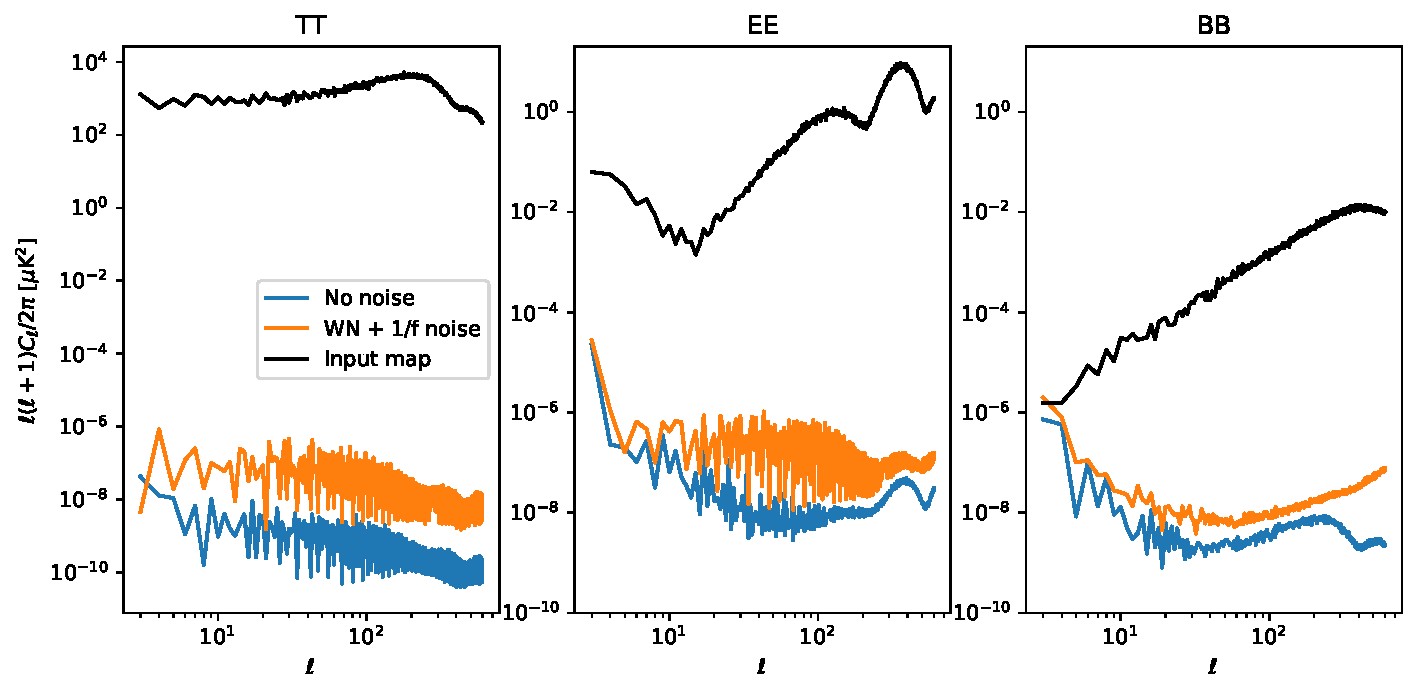
\includegraphics[width=0.7\textwidth]{images/calibration_spectra.pdf}
\caption{\label{fig:calibration_spectra} Residual power due to calibration.}
\end{figure}
%------------------------------------------------------------------------------------------

Photometric calibration is the process of converting the raw output of the receivers into astrophysical units via the characterization of the \emph{gain factor} $G(t)$ which we allow to vary with time.  In space, the characterization of $G(t)$ uses the dipole.   For the PICO concept study, we evaluated the impact of noise in the estimation of $G(t)$ using the tools developed for the Planck/LFI instrument and the CORE mission proposal. The quality of the estimate depends on the noise level of the receivers, but also on the details of the scanning strategy. 
To analyze the impact of calibration uncertainties on PICO, we performed  the following analysis:1. We simulated the observation of the sky, assuming four receivers, the nominal scanning strategy, and $1/f$ noise. The simulated sky contained CMB anisotropies, plus the CMB dipole. 2. We ran the calibration code to fit the dipole against the raw data simulated during step~1. 3. We again simulated the observation of the sky, this time using the values of $G$ computed during step~2, which contain errors due to the presence of noise and the CMB signal.

The presence of large-scale Galactic emission features can bias the estimation of calibration factors. Ideally, a full data analysis pipeline would pair the calibration step with the component separation step, following a schema similar to Planck/LFI's legacy data processing\cite{Planck2018_II}: the calibration code is followed by a component separation analysis, and these two steps are iterated until the solution converges.

Results of the simulation (neglecting foregrounds) are shown as power spectrum residuals in Fig.~\ref{fig:calibration_spectra}. 
We estimate the gain fluctuations to better than 10$^{-4}$ solving for the gain every 40 hours (4 precession periods).
The scanning strategy employed by PICO allows for a much better calibration than Planck, thanks to the much faster precession.

\subsubsection{Far Sidelobe Pickup}
\label{sec:fsl}
%The main beam (within a few degrees of the axis of beam response) in a CMB mission can be measured to high precision using the planets .  
Measurement of each detector's response to signals off axis, which tends to be weak (--80dB less than the peak response) but spread over a very large solid angle, is difficult to do pre-launch, and may not even be done accurately after launch.  Nonetheless, this far sidelobe can couple bright Galactic signal from many tens of degrees off-axis and confuse it with polarized signal from the CMB off the Galactic plane.  

To evaluate this systematic error, GRASP software\footnote{https://www.ticra.com} was used to compute the \pico\ telescope's response over the full sky.  This full-sky beam was convolved with a polarized Galactic signal and a full \pico\ mission scan using the simulation pipeline.  The far sidelobe pickup was estimated to contribute less than XXX to the B-mode angular power spectrum and thus an error in $r$ of YYY.

Due to the difficulties of measuring this beam, physical optics simulation capabilities must be maintained and validated as well as possible with on-orbit data.

\subsubsection{Key Findings}
Properly modeling, engineering for, and controlling the effects of systematic errors in a
next-generation CMB probe is critical.  As of today, we conclude that there is a clear path to demonstrate that state-of-the-art technology and data processing can take advantage of the L2 environment and control systematic errors to a level that enables the science goals of PICO. In particular we note:
\begin{itemize}
\item The raw sensitivity of the instrument should include enough margin
that data subsets can independently achieve the science goals.
This allows testing of the results in the data analysis and additional
data cuts, if needed.

\item NASA's support of ground-based and suborbital CMB missions will mitigate risk to a future space mission as PICO by continuing to develop analysis techniques and technology for mitigation of systematic errors.

\item In a PICO mission's phase A, a complete end-to-end system-level
simulation software facility would be developed to assist the team in setting 
requirements and conducting trades between subsystem requirements while
realistically accounting for post-processing mitigation.  Any future
CMB mission is likely to have similar orbit  
and scan characteristics to those of PICO, thus there is an opportunity for NASA and
the CMB community to invest in further development of this capability now.
\end{itemize}

\end{document}

%\begin{figure}[!htb]
%\centering
%
\includegraphics[width=4cm]{images/example}
%\caption{example}
%\label{fig:im_3}
%\end{figure}
